\chapter{Self-Gravitating Gas}
\label{ch:selfgrav}

A cold cloud of molecular gas in the Galaxy is tens of parsecs across and about $10\,\mathrm K$ (Table~\ref{tab:ism_cloud_types}). Some such clouds sit unchanged for millions of years. Others break up into dense cores that shrink, heat up and become stars. Three things decide which. Gravity pulls every part of the cloud toward every other part. Pressure pushes back. Rotation, small at first, resists being squeezed sideways.

Pressure is not one thing. In a star it is a sum,
\[
P=P_{\rm gas}+P_{\rm light}+P_{\rm degenerate}+\cdots,
\]
and each term is one case of counting states (P3, Section~\ref{pr:sec:p3}). Gas pressure holds up the Sun over most of its interior. Light carries a growing share in more massive stars (Problem~\ref{pr:prob:prad}). Degenerate electrons hold up white dwarfs. In a planet the pressure comes instead from compressed liquid and solid, each with its own equation of state.

Two questions run through what follows. When does gravity win, and why does a body held together by gravity get hotter when it loses energy?

% ==============================================================================
\section{Hydrostatic Equilibrium}
\label{sg:sec:hse}

Chapter~\ref{ch:principles} gave the Euler equation for any moving gas (P1, Eq.~\eqref{pr:eq:euler}) and the pull of a sphere on its own parts (P2, Eq.~\eqref{pr:eq:shell_theorem}).

A star that shines for billions of years is not speeding up or slowing down anywhere inside. The full Euler equation carries terms for motion that such a star does not need.

Think of a pile of books. The bottom book carries the weight of every book above it. The one in the middle carries half the pile. A diver feels the same thing in water. Every ten metres of depth adds the weight of ten metres of water above each square metre, about one atmosphere.

Inside a star each layer holds up all the layers above it, so the pressure must grow toward the centre. At every radius the pressure difference across a thin layer balances the weight of that layer. This is momentum conservation (P1) for gas at rest, with the gravity of a sphere (P2).

The diver in numbers. Water has $\rho=1000\,\mathrm{kg\,m^{-3}}$ and $g=9.8\,\mathrm{m\,s^{-2}}$, so the pressure grows by $\rho g=9800\,\mathrm{Pa}$ per metre, and one atmosphere, $1.01\times10^5\,\mathrm{Pa}$, every $10.3\,\mathrm m$.

The picture is a thin slab of gas with more pressure pushing up on its bottom face than down on its top face. The difference is exactly its weight.

The same balance sets how fast the air thins with height, how thick a disk of gas around a star is, and how much mass a galaxy cluster must have to hold its hot gas (Problem~\ref{sg:prob:cluster}). It gives the pressure gradient at every radius of a star.

\paragraph{The equation.} Set $\vec v=0$ in the Euler equation \eqref{pr:eq:euler} and use the gravity of a sphere \eqref{pr:eq:shell_theorem}. Only the radial component survives,
\begin{align}
	0
	&\eqby{1} -\nabla P+\rho\,\vec g \nonumber\\
	&\eqby{2} -\dv{P}{r}\,\rhat-\rho\,\frac{G\,m(r)}{r^2}\,\rhat .
\end{align}
\begin{explain}
	\item Eq.~\eqref{pr:eq:euler} with $\vec v=0$ everywhere and at all times.
	\item Spherical symmetry, so $P$ depends only on $r$, and $\vec g$ from Eq.~\eqref{pr:eq:shell_theorem}.
\end{explain}
\begin{equation}
	\boxed{\dv{P}{r}=-\frac{G\,m(r)\,\rho}{r^2}.}
	\label{sg:eq:hse}
\end{equation}
This is \textbf{hydrostatic equilibrium}. It holds for any star at rest, whatever its equation of state and whatever carries its energy. It does not say what $P$ is made of.

\paragraph{How large is the central pressure?} Replace the derivative by the drop of the pressure from the centre to the surface, $-P_c/R$, and put the whole mass at a typical radius $R$. Then $P_c\sim GM^2/R^4$. For the Sun this is $1.1\times10^{15}\,\mathrm{Pa}$. The detailed models of Chapter~\ref{ch:structure} give $2.5\times10^{16}\,\mathrm{Pa}$, larger because the Sun's mass is concentrated toward its centre. The estimate gets the size right to within a factor of a few without any knowledge of what the Sun is made of.

\paragraph{An atmosphere.} Near the surface of a planet, $m(r)$ and $r$ hardly change, so $Gm/r^2$ is the constant surface gravity $g$. If the air is an ideal gas at one temperature $T$, with mean mass $\mu m_{\rm H}$ per particle, Eq.~\eqref{pr:eq:ideal_gas} gives $\rho=P\,\mu m_{\rm H}/(k_BT)$. With height $z$ in place of $r$,
\begin{align}
	\dv{P}{z}
	&\eqby{1} -\rho g \nonumber\\
	&\eqby{2} -\frac{\mu m_{\rm H}\,g}{k_BT}\,P ,
\end{align}
\begin{explain}
	\item Eq.~\eqref{sg:eq:hse} with $Gm/r^2=g$ held constant.
	\item The ideal-gas law solved for $\rho$.
\end{explain}
so the pressure falls exponentially,
\begin{equation}
	P(z)=P(0)\,e^{-z/H},\qquad H=\frac{k_BT}{\mu m_{\rm H}\,g}.
	\label{sg:eq:scale_height}
\end{equation}
The \textbf{scale height} $H$ is the height over which the pressure falls by a factor $e$. For the Earth's air ($T=288\,\mathrm K$, mean molecular mass $28.97$ atomic mass units) it is $8.4\,\mathrm{km}$. A hotter or lighter gas reaches higher.

\paragraph{Planets, and why their interiors are layered.} A planet obeys Eq.~\eqref{sg:eq:hse} just as a star does, but its pressure comes from rock, ice and liquid rather than from hot gas and light. Gravity does not change these materials directly. It compresses them. Going down, the pressure grows as Eq.~\eqref{sg:eq:hse} demands, and usually the temperature grows with it, so each depth sits at a different point $(P,T)$ of the material's phase diagram. Where that point crosses a phase boundary, the stable form of the material changes. Rock turns into denser mineral structures, and in the giant planets hydrogen is squeezed into a dense, metallic state. A layered interior is hydrostatic equilibrium plus a phase diagram.

% ==============================================================================
\section{The Virial Theorem}
\label{sg:sec:virial}

Hydrostatic equilibrium gives the pressure at every radius, but only once the density at every radius is known. That needs the equation of state and the way energy flows, which is the work of Chapter~\ref{ch:structure}.

Often the profile is not wanted at all. The questions are simpler. How hot is a star, on average? How much energy does it hold? What happens to it when it loses some?

Think of a satellite in a circular orbit. The lower its orbit, the faster it moves. A satellite that skims the air feels a little drag, loses energy, and sinks to a lower orbit, where it moves faster. Losing energy has sped it up. The station at $400\,\mathrm{km}$ moves at $7.67\,\mathrm{km\,s^{-1}}$. Dropped to $300\,\mathrm{km}$ it would move at $7.73\,\mathrm{km\,s^{-1}}$.

The particles of a star are like satellites in the star's own gravity. Averaged over the whole star, their kinetic energy is tied to the depth of the gravitational well in the same way. Since the kinetic energy of a gas measures its temperature, the depth of the well sets the temperature. This is the virial theorem. It is hydrostatic equilibrium (P1 and P2) added up over the whole star, read with P3.

The satellite in symbols. Gravity supplies the centripetal force, $m v^2/r=GMm/r^2$. So the kinetic energy is $K=\tfrac12mv^2=GMm/(2r)$ and the potential energy is $U=-GMm/r$. Then $2K+U=0$, and the total energy is $E=K+U=-K$, the result $E=-GM\mu/2a$ of Eq.~\eqref{eq:visviva_E} for a circular orbit. Lowering $E$ raises $K$.

The picture is a bowl. The deeper the bowl, the faster everything in it has to move to stay in it.

The same theorem is Clausius's virial of a gas. Zwicky applied it to the galaxies of the Coma cluster and found that they move far too fast for the mass that shines, the first evidence of dark matter. It turns the speeds of stars into the mass of a galaxy, and the temperature of the hot gas in a cluster into the cluster's mass. Here it gives the theorem for a gas sphere by two routes, the temperature of a star, and how firmly a star is bound.

\paragraph{Route A, from hydrostatic equilibrium.} Multiply Eq.~\eqref{sg:eq:hse} by $4\pi r^3$ and integrate from the centre to the surface $R$. On the left,
\begin{align}
	\int_0^R4\pi r^3\,\dv{P}{r}\,dr
	&\eqby{1} \Big[4\pi r^3P\Big]_0^R-3\int_0^R4\pi r^2P\,dr \nonumber\\
	&\eqby{2} -3\int P\,dV .
\end{align}
\begin{explain}
	\item Integration by parts.
	\item At the centre $r^3=0$, and at the surface $P=0$. The volume element is $dV=4\pi r^2dr$.
\end{explain}
On the right,
\begin{align}
	\int_0^R4\pi r^3\left(-\frac{Gm\rho}{r^2}\right)dr
	&\eqby{1} -\int_0^M\frac{Gm}{r}\,dm \nonumber\\
	&\eqby{2} U .
\end{align}
\begin{explain}
	\item $4\pi r^2\rho\,dr=dm$, Eq.~\eqref{pr:eq:mass_inside}.
	\item The gravitational energy, Eq.~\eqref{pr:eq:U_def}.
\end{explain}
Setting the two equal,
\begin{equation}
	\boxed{3\int P\,dV+U=0.}
	\label{sg:eq:virial_P}
\end{equation}
Only gravity and the pressure enter, so this holds for any equation of state. It is hydrostatic equilibrium weighted by $r$ and summed over the star. The detail at each radius is lost, and the overall balance is kept.

\paragraph{Route B, for a gas that moves.} Route A assumed the gas is at rest. To see what happens when it is not, follow the second moment of the mass, $I\equiv\int r^2\,dm$, where each $dm$ moves with the gas. Differentiating twice,
\begin{align}
	\frac12\dv[2]{I}{t}
	&\eqby{1} \int v^2\,dm+\int\vecr\cdot\dv{\vec v}{t}\,dm \nonumber\\
	&\eqby{2} 2K_{\rm bulk}+\int\vecr\cdot\big(-\nabla P+\rho\,\vec g\big)\,dV \nonumber\\
	&\eqby{3} 2K_{\rm bulk}+3\int P\,dV+U .
\end{align}
\begin{explain}
	\item $\dv*{(r^2)}{t}=2\vecr\cdot\vec v$, then once more. The mass elements do not change (P1).
	\item $K_{\rm bulk}=\tfrac12\int v^2\,dm$ is the kinetic energy of bulk motion. The Euler equation \eqref{pr:eq:euler} gives $\rho\,\dv*{\vec v}{t}$.
	\item $-\int\vecr\cdot\nabla P\,dV=3\int P\,dV$ by integration by parts, as in Route A. For a sphere, $\vecr\cdot\vec g=-Gm/r$ by Eq.~\eqref{pr:eq:shell_theorem}, so the gravity term is $U$ as in Route A. (For any shape the same result follows by writing $U$ as a double sum over pairs of mass elements.)
\end{explain}
For a gas of slow particles, $\gamma=\tfrac53$ in Eq.~\eqref{pr:eq:P_u}, so $\int P\,dV=\tfrac23K_{\rm th}$, where $K_{\rm th}$ is the kinetic energy of the random thermal motion. With the total kinetic energy $K=K_{\rm bulk}+K_{\rm th}$,
\begin{equation}
	\boxed{\frac12\dv[2]{I}{t}=2K+U.}
	\label{sg:eq:virial_dynamic}
\end{equation}
A cloud that neither grows nor shrinks on average has $\avg{\ddot I}=0$, and $2K+U=0$, which is Route A again. If $2K<|U|$, then $\ddot I<0$. The cloud's size accelerates inward and it collapses. If $2K>|U|$, it disperses.

\paragraph{Reading it, gravity sets the temperature.} Let the gas be ideal with mean mass $\mu m_{\rm H}$ per particle, where $\mu$ is the \textbf{mean molecular weight}, so that the number density is $n=\rho/(\mu m_{\rm H})$. Then
\[
\int P\,dV=\int nk_BT\,dV=\frac{k_B}{\mu m_{\rm H}}\int T\,dm\equiv\frac{Mk_B\bar T}{\mu m_{\rm H}},
\]
which defines $\bar T$, the temperature averaged over the mass. With Eq.~\eqref{sg:eq:virial_P},
\begin{equation}
	\boxed{k_B\bar T=\frac{\mu m_{\rm H}\,|U|}{3M}.}
	\label{sg:eq:virial_T}
\end{equation}
The average temperature of a star is set by the depth of its gravitational well per unit mass, and by nothing else. The source of its energy does not appear.

\paragraph{A uniform sphere.} To put numbers in, take a sphere of uniform density. The mass inside $r$ is $m=M(r/R)^3$, so $dm=3Mr^2dr/R^3$, and Eq.~\eqref{pr:eq:U_def} gives
\begin{align}
	U
	&\eqby{1} -\int_0^R\frac{G\,M(r/R)^3}{r}\,\frac{3Mr^2}{R^3}\,dr \nonumber\\
	&\eqby{2} -\frac{3GM^2}{R^6}\int_0^Rr^4\,dr \nonumber\\
	&= -\frac35\,\frac{GM^2}{R} .
	\label{sg:eq:U_uniform}
\end{align}
\begin{explain}
	\item Eq.~\eqref{pr:eq:U_def} with $m=M(r/R)^3$ and $dm=3Mr^2dr/R^3$.
	\item Collect the powers of $r$ and $R$.
\end{explain}
Then Eq.~\eqref{sg:eq:virial_T} becomes $k_B\bar T=G M\mu m_{\rm H}/(5R)$. For the Sun, with $\mu=0.6$ for its ionised gas, this is $\bar T=2.8\times10^6\,\mathrm K$. The real Sun is denser toward the middle, so its well is deeper and its gas hotter. Its centre is at $1.57\times10^7\,\mathrm K$. Without knowing anything about nuclear fusion, the virial theorem says that the inside of the Sun is at millions of kelvin. That is hot enough for hydrogen nuclei to fuse (Section~\ref{st:sec:eos}), which is why stars shine by fusion at all.

\paragraph{How firmly a star is bound.} Let the gas have $P=(\gamma-1)u$, Eq.~\eqref{pr:eq:P_u}. Its internal energy is $\int u\,dV=\int P\,dV/(\gamma-1)$, and the total energy is
\begin{align}
	E
	&\eqby{1} \frac{1}{\gamma-1}\int P\,dV+U \nonumber\\
	&\eqby{2} -\frac{U}{3(\gamma-1)}+U \nonumber\\
	&= \frac{3\gamma-4}{3(\gamma-1)}\,U .
\end{align}
\begin{explain}
	\item Internal energy plus gravitational energy, for a star at rest.
	\item The virial theorem \eqref{sg:eq:virial_P}, $\int P\,dV=-U/3$.
\end{explain}
\begin{equation}
	\boxed{E=\frac{3\gamma-4}{3(\gamma-1)}\,U.}
	\label{sg:eq:E_gamma}
\end{equation}
For slow particles, $\gamma=\tfrac53$ and $E=U/2<0$. The star is bound, and taking it apart costs half its gravitational energy. As $\gamma\to\tfrac43$, $E\to0$. The star is barely bound, and a small push can make it collapse or fly apart. For $\gamma<\tfrac43$ no static balance exists at all. This single line explains three later results. Stars held up mainly by light are fragile (Section~\ref{st:sec:polytropes}). White dwarfs whose electrons move near the speed of light have a maximum mass (Section~\ref{cs:sec:wd}). And a collapsing protostar collapses a second time while its molecules are being broken apart (Section~\ref{sg:sec:rotation}).

% ==============================================================================
\section{Negative Heat Capacity}
\label{sg:sec:negheat}

By the virial theorem a star of slow particles has $E=-K$, Eq.~\eqref{sg:eq:E_gamma} with $\gamma=\tfrac53$.

Everyday thermodynamics says that something that loses heat gets colder. Its heat capacity, the energy needed to raise its temperature by one kelvin, is positive. A star seems to break this rule.

Think of a cup of tea left in a room. It cools until it has the temperature of the room, and then its energy wobbles a little around a fixed value as the room's air gives and takes small amounts of heat. The room decides the temperature. The rule that heat capacity is positive is a statement about objects that sit in a room like this, with a large surrounding body that sets the temperature.

A star has no room around it. It is isolated in empty space, held together by its own gravity, and it loses energy only by radiating into space, which never sends heat back. Nothing sets its temperature from outside. Its temperature follows from its energy through the virial theorem, and that relation runs backwards. The proof that heat capacity is positive does not apply to it.

The Sun in numbers. With $\mu=0.6$ the Sun holds $N=M/(\mu m_{\rm H})=2.0\times10^{57}$ particles, and $E=-K=-\tfrac32Nk_B\bar T$. If it shone at its present luminosity for a million years with no fusion, it would lose $\Delta E=-1.2\times10^{40}\,\mathrm J$, and its mean temperature would rise by $3\times10^5\,\mathrm K$.

The picture is a curve of temperature against energy that slopes the wrong way. Moving left along it, toward lower energy, the temperature climbs.

The same behaviour appears in the core collapse of globular star clusters and in black holes, whose temperature rises as they lose mass to Hawking radiation. It gives the sign of the heat capacity of a star, the reason the usual rule fails, and what a negative heat capacity does for a star.

\paragraph{The heat capacity of a star.} Along a sequence of stars in virial balance, each with a slightly different energy, $E=-\tfrac32Nk_B\bar T$. So
\begin{equation}
	\boxed{C\equiv\dv{E}{\bar T}=-\frac32Nk_B<0.}
	\label{sg:eq:negative_C}
\end{equation}
Losing energy by radiation, $dE<0$, raises the temperature, $d\bar T=dE/C>0$. Of the gravitational energy released by contraction, half goes into heating the gas and half is radiated away, since $\Delta K=-\Delta U/2$ and $\Delta E=\Delta U/2$.

\paragraph{Why the usual rule says $C\ge0$.} The usual rule belongs to the canonical ensemble, a system in contact with a heat bath at temperature $T$. With $\beta=1/k_BT$ its partition function is $Z(\beta)=\sum_se^{-\beta E_s}$, summed over its states $s$. The mean energy and its spread follow from $Z$,
\begin{align}
	\avg{E}
	&\eqby{1} -\pdv{\ln Z}{\beta}, \nonumber\\
	\avg{(\Delta E)^2}=\avg{E^2}-\avg{E}^2
	&\eqby{2} \pdv[2]{\ln Z}{\beta}
	\eqby{3} -\pdv{\avg{E}}{\beta}
	\eqby{4} k_BT^2\,\pdv{\avg{E}}{T}.
\end{align}
\begin{explain}
	\item Differentiate $\ln Z$ once. Each state enters with weight $e^{-\beta E_s}/Z$.
	\item Differentiate once more. The second derivative of $\ln Z$ is the mean of $E^2$ minus the square of the mean of $E$.
	\item The first line.
	\item $\beta=1/k_BT$, so $\partial/\partial\beta=-k_BT^2\,\partial/\partial T$.
\end{explain}
\begin{equation}
	\boxed{C_{\rm can}=\frac{\avg{(\Delta E)^2}}{k_BT^2}\ge0.}
	\label{sg:eq:canonical_C}
\end{equation}
A spread in energy cannot be negative, so in contact with a bath the heat capacity cannot be negative either. This is a statement about the canonical ensemble only.

\paragraph{The isolated system.} An isolated star has a fixed energy and belongs to the microcanonical ensemble, where the temperature is defined from the entropy $S(E)$ by $1/T=\dv*{S}{E}$. Comparing neighbouring equilibria with slightly different $E$,
\begin{align}
	\dv{E}\left(\frac1T\right)
	&\eqby{1} \dv[2]{S}{E} \nonumber\\
	\implies\quad -\frac{1}{T^2}\,\dv{T}{E}
	&= \dv[2]{S}{E} \nonumber\\
	\implies\quad C_{\rm micro}=\dv{E}{T}
	&\eqby{2} -\frac{1}{T^2\,\dv*[2]{S}{E}} .
\end{align}
\begin{explain}
	\item Differentiate the definition of $T$ once more.
	\item Invert $\dv*{T}{E}$.
\end{explain}
Nothing here forbids $C<0$. It only requires $\dv*[2]{S}{E}>0$, an entropy that curves upward. For short-range forces, a large system can be split into parts whose energies add, and then the two ensembles agree and $S(E)$ curves downward. Gravity is long-range. The energy of a star is not the sum of the energies of its halves, because the halves attract each other. So the two ensembles need not agree, and a self-gravitating body can have $C<0$ as an isolated system even though no system with $C<0$ can sit in steady contact with a bath.

That last point is itself physical. Put a star in a bath slightly hotter than itself. Heat flows in, and with $C<0$ the star cools, so even more heat flows in. Put it in a slightly cooler bath and it heats as it loses heat. Either way it runs away from the bath's temperature. A self-gravitating body cannot come into steady equilibrium with a heat bath.

\paragraph{What it does for a star.} Suppose the nuclear burning in a core runs a little too fast. The extra energy expands the core, and by Eq.~\eqref{sg:eq:negative_C} the core cools, which slows the burning. If the burning runs too slow, the core contracts and heats until the burning catches up. Negative heat capacity makes a star its own thermostat (P4 on the energy, Section~\ref{pr:sec:p4}). When fuel runs out in the core, the same rule makes the core contract and heat until the next fuel ignites. Where the pressure stops depending on temperature, in degenerate matter, the thermostat breaks, and burning can run away (Section~\ref{st:sec:eos}).

% ==============================================================================
\section{The Jeans Criterion}
\label{sg:sec:jeans}

The virial theorem says when a whole cloud is in balance, $2K+U=0$, and that it collapses when $2K<|U|$.

It does not say which parts of a large cloud collapse, or how big the pieces are.

Think of traffic on a busy road. Now and then cars bunch up a little. Drivers in a bunch slow down, the cars behind catch up, and the bunch grows. Drivers also react and spread out again. A short bunch is smoothed out before it can grow. A long one grows faster than drivers can spread it, and becomes a jam. Only bunches longer than some length grow.

A cloud behaves the same way. A region that is slightly denser than its surroundings pulls in more gas. Its higher pressure pushes back, and that push travels at the speed of sound. A small region is smoothed out by sound before gravity can act. A large region collapses before sound can cross it. The dividing size, where the sound-crossing time equals the free-fall time, is the Jeans length. This is a comparison of two scales (P6), made exact with conservation (P1) and the gravity of the gas (P2).

A dense core in numbers. Molecular gas at $10\,\mathrm K$ with $n=10^{10}\,\mathrm{m^{-3}}$ ($10^4\,\mathrm{cm^{-3}}$) and $\mu=2.33$ has the sound speed $c_s=\sqrt{k_BT/(\mu m_{\rm H})}=188\,\mathrm{m\,s^{-1}}$ and the free-fall time $t_{\rm ff}=3.4\times10^5$ years (Section~\ref{sg:sec:freefall}). In that time sound covers $c_st_{\rm ff}=0.065\,\mathrm{pc}$. Regions much larger than this cannot be held up.

The picture is Figure~\ref{sg:fig:jeans}. Short waves oscillate as ordinary sound. Long waves do not oscillate at all. They grow.

\begin{figure}[htbp]
	\centering
	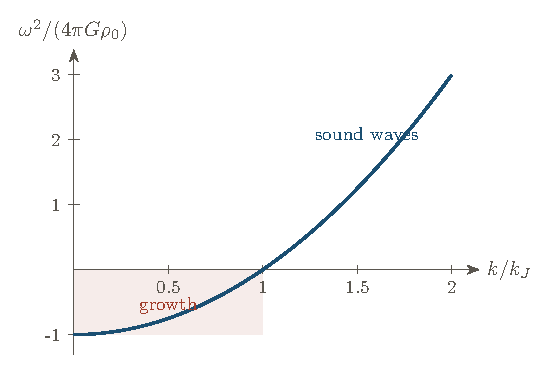
\includegraphics{fig_ch10_jeans_dispersion.pdf}
	\caption{The squared frequency $\omega^2$ of a small wave in a uniform self-gravitating gas against its wavenumber $k$, in units of $4\pi G\rho_0$ and of $k_J$. Below $k=k_J$ (shaded) $\omega^2<0$.}
	\label{sg:fig:jeans}
\end{figure}

The same instability, with the expansion of the universe added, grows the galaxies and clusters out of the nearly smooth early universe. In a rotating disk it becomes the Toomre criterion for spiral arms and clumps. It gives the critical mass and length, by energy and by waves.

\paragraph{By energy.} Take a uniform sphere of mass $M$, radius $R$ and temperature $T$. Its thermal energy is $K=\tfrac32Nk_BT=\tfrac32Mk_BT/(\mu m_{\rm H})$ (Eq.~\eqref{pr:eq:ideal_gas}), and its gravitational energy is Eq.~\eqref{sg:eq:U_uniform}. The marginal case of Eq.~\eqref{sg:eq:virial_dynamic}, $2K=|U|$, gives
\begin{align}
	3\,\frac{Mk_BT}{\mu m_{\rm H}}
	&= \frac35\,\frac{GM^2}{R} \nonumber\\
	\implies\quad R
	&= \frac{G M\mu m_{\rm H}}{5k_BT} .
\end{align}
Writing $M=\tfrac43\pi R^3\rho$ and eliminating $R$ or $M$ gives the \textbf{Jeans mass} and \textbf{Jeans length},
\begin{equation}
	\boxed{M_J=\left(\frac{5k_BT}{G\mu m_{\rm H}}\right)^{3/2}\left(\frac{3}{4\pi\rho}\right)^{1/2},\qquad
	R_J=\left(\frac{15\,k_BT}{4\pi G\mu m_{\rm H}\rho}\right)^{1/2}.}
	\label{sg:eq:jeans_mass}
\end{equation}
A cloud with $M>M_J$ cannot be held up by its thermal pressure. For the dense core above, $M_J=5.4\,M_\odot$ and $R_J=0.13\,\mathrm{pc}$. Hot, thin gas is stable. Cold, dense gas is not, which is why stars form in cold molecular clouds rather than in the warm diffuse gas.

\paragraph{By waves.} Take an infinite gas at rest with uniform density $\rho_0$ and one temperature, so that a small change of density $\rho_1$ changes the pressure by $c_s^2\rho_1$. Disturb it slightly, $\rho=\rho_0+\rho_1$, $\vec v=\vec v_1$, $\Phi=\Phi_0+\Phi_1$. To first order in the small quantities, continuity \eqref{pr:eq:continuity}, Euler \eqref{pr:eq:euler} and Poisson \eqref{pr:eq:poisson} read
\begin{equation}
	\pdv{\rho_1}{t}+\rho_0\nabla\cdot\vec v_1=0,\qquad
	\rho_0\pdv{\vec v_1}{t}=-c_s^2\nabla\rho_1-\rho_0\nabla\Phi_1,\qquad
	\nabla^2\Phi_1=4\pi G\rho_1 .
\end{equation}
(Strictly, a uniform $\rho_0$ cannot be at rest, because Poisson's equation then needs a $\Phi_0$ that grows without bound. Jeans set this aside, and the result is still right for regions much smaller than the cloud.) For a wave $\propto e^{i(kx-\omega t)}$ along $x$, with $\vec v_1=v_1\hat x$, each derivative becomes a factor, $\partial_t\to-i\omega$ and $\partial_x\to ik$. The three equations become one matrix equation for the three amplitudes,
\begin{equation}
	\begin{pmatrix}
		-i\omega & i\rho_0k & 0\\
		ic_s^2k & -i\omega\rho_0 & i\rho_0k\\
		4\pi G & 0 & k^2
	\end{pmatrix}
	\begin{pmatrix}\rho_1\\ v_1\\ \Phi_1\end{pmatrix}=0 .
	\label{sg:eq:jeans_matrix}
\end{equation}
A wave exists only if the determinant vanishes,
\begin{align}
	0
	&\eqby{1} -i\omega\big(-i\omega\rho_0k^2\big)-i\rho_0k\big(ic_s^2k^3-i\rho_0k\cdot4\pi G\big) \nonumber\\
	&\eqby{2} \rho_0k^2\big(c_s^2k^2-4\pi G\rho_0-\omega^2\big).
\end{align}
\begin{explain}
	\item Expand along the first row.
	\item Multiply out, using $i^2=-1$, and collect.
\end{explain}
\begin{equation}
	\boxed{\omega^2=c_s^2k^2-4\pi G\rho_0.}
	\label{sg:eq:jeans_dispersion}
\end{equation}
Short waves, with large $k$, have $\omega^2>0$ and oscillate as sound. Long waves with $k$ below $k_J=\sqrt{4\pi G\rho_0}/c_s$ have $\omega^2<0$, so $\omega$ is imaginary and the disturbance grows exponentially instead of oscillating. The critical wavelength is
\begin{equation}
	\lambda_J=\frac{2\pi}{k_J}=c_s\sqrt{\frac{\pi}{G\rho_0}} .
	\label{sg:eq:jeans_wavelength}
\end{equation}
It scales with $T$ and $\rho$ exactly as $R_J$ does, and differs only in the number in front, because one route treats a finite sphere and the other an infinite medium. Both say $\lambda_J\approx c_s\,t_{\rm ff}$. With $t_{\rm ff}$ from Eq.~\eqref{sg:eq:tff} the ratio is $\sqrt{32/3}=3.3$.

\paragraph{Why stars form in groups.} A giant molecular cloud holds $10^5$ to $10^6\,M_\odot$ (Table~\ref{tab:ism_cloud_types}), many thousands of Jeans masses. It does not collapse into one star. While it collapses it stays thin enough to radiate away the heat of compression, so its temperature stays near $10\,\mathrm K$. By Eq.~\eqref{sg:eq:jeans_mass}, $M_J\propto T^{3/2}\rho^{-1/2}$ then falls as the density rises, so parts that were stable become unstable on their own. The cloud breaks into clumps, the clumps into cores, and each core into stars. This is why most stars are born in clusters and in pairs, although many clusters later drift apart.

% ==============================================================================
\section{Free Fall and the Three Clocks}
\label{sg:sec:freefall}

The Jeans criterion says when a region collapses.

It does not say how fast.

Imagine a hole drilled straight through a uniform Earth. A ball dropped into it reaches the centre after $21$ minutes, whatever the hole's length. The time depends only on the Earth's density, as the units of $G\rho$ demand (Section~\ref{pr:sec:p6}).

A cloud whose pressure can no longer resist gravity falls in on itself in the same way. Each shell falls toward the centre pulled by the mass inside it. The time to reach the centre depends only on the density, so every shell of a uniform cloud arrives at the same moment. This is conservation of energy (P1) for each shell, with the gravity of a sphere (P2).

A uniform cloud with the Earth's mean density would collapse in $15$ minutes. The Sun's mean density gives $30$ minutes. A dense core of a molecular cloud takes $3.4\times10^5$ years.

The picture is Figure~\ref{sg:fig:freefall}. The radius falls slowly at first and then plunges to zero.

\begin{figure}[htbp]
	\centering
	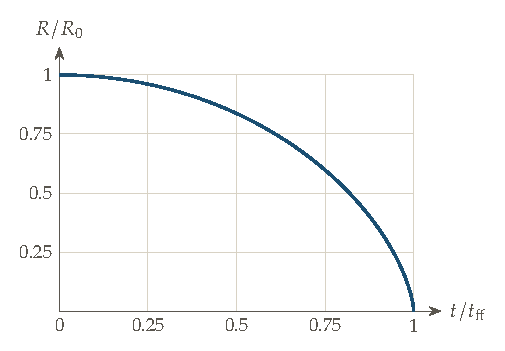
\includegraphics{fig_ch10_freefall.pdf}
	\caption{The radius of a shell in a uniform, pressure-free sphere that starts at rest, against time in units of the free-fall time.}
	\label{sg:fig:freefall}
\end{figure}

The same collapse is a Kepler orbit with no angular momentum (Chapter~\ref{ch:twobody}). In cosmology it is the collapse of a uniform overdense sphere into a galaxy halo, and in a massive star it sets how fast the core falls in at the start of a supernova. It gives the free-fall time and the three clocks of a star.

\paragraph{The fall of one shell.} Take a uniform cloud of density $\rho_0$ at rest, with no pressure. Follow a shell that starts at radius $R_0$, with mass $M=\tfrac43\pi R_0^3\rho_0$ inside it. While the shells do not cross, $M$ stays the same, and by Eq.~\eqref{pr:eq:shell_theorem}
\begin{equation}
	\dv[2]{R}{t}=-\frac{GM}{R^2}.
\end{equation}
Multiplying by $\dv*{R}{t}$ and integrating from rest at $R_0$ gives the energy of the shell per unit mass,
\begin{align}
	\frac12\left(\dv{R}{t}\right)^2-\frac{GM}{R}
	&= -\frac{GM}{R_0} \nonumber\\
	\implies\quad \left(\dv{R}{t}\right)^2
	&= \frac{2GM}{R_0}\left(\frac{R_0}{R}-1\right).
\end{align}
The substitution $R=R_0\cos^2\xi$, with $\xi$ running from $0$ at the start to $\pi/2$ at the centre, turns the bracket into $\tan^2\xi$,
\begin{align}
	\Big(-2R_0\cos\xi\sin\xi\,\dv{\xi}{t}\Big)^2
	&\eqby{1} \frac{2GM}{R_0}\,\frac{\sin^2\xi}{\cos^2\xi} \nonumber\\
	\implies\quad \cos^2\xi\,\dv{\xi}{t}
	&\eqby{2} \sqrt{\frac{GM}{2R_0^3}} \nonumber\\
	\implies\quad \xi+\sin\xi\cos\xi
	&\eqby{3} \sqrt{\frac{2GM}{R_0^3}}\;t .
\end{align}
\begin{explain}
	\item $\dv*{R}{t}=-2R_0\cos\xi\sin\xi\,\dv*{\xi}{t}$, and $R_0/R-1=1/\cos^2\xi-1=\tan^2\xi$.
	\item Divide both sides by $4R_0^2\sin^2\xi$ and take the positive root, since $\xi$ grows.
	\item $\int_0^\xi2\cos^2\xi'\,d\xi'=\xi+\sin\xi\cos\xi$, with $\xi=0$ at $t=0$.
\end{explain}
The shell reaches the centre at $\xi=\pi/2$. With $M=\tfrac43\pi R_0^3\rho_0$, $\sqrt{2GM/R_0^3}=\sqrt{8\pi G\rho_0/3}$, and
\begin{equation}
	\boxed{t_{\rm ff}=\frac{\pi/2}{\sqrt{8\pi G\rho_0/3}}=\sqrt{\frac{3\pi}{32\,G\rho_0}}.}
	\label{sg:eq:tff}
\end{equation}
$R_0$ has dropped out. Every shell of a uniform cloud reaches the centre at the same time, so shells never cross, which is what the calculation assumed. The time is $(G\rho_0)^{-1/2}$ times a number, as P6 said it must be.

\paragraph{The same result as a Kepler orbit.} A shell falling from rest is a body on a Kepler orbit of zero angular momentum. As the angular momentum shrinks to zero at fixed energy, the ellipse of Chapter~\ref{ch:twobody} flattens into a straight segment from $R_0$ to the centre, with semi-major axis $R_0/2$. The fall from one end to the other is half an orbital period. By Eq.~\eqref{eq:kepler3},
\[
t_{\rm ff}=\frac12\cdot2\pi\sqrt{\frac{(R_0/2)^3}{GM}}=\pi\sqrt{\frac{R_0^3}{8GM}}=\sqrt{\frac{3\pi}{32\,G\rho_0}},
\]
the same as Eq.~\eqref{sg:eq:tff}.

\paragraph{The three clocks of a star.} A star changes on three very different times.
\begin{itemize}
	\item The \textbf{free-fall} or dynamical time, Eq.~\eqref{sg:eq:tff}. It is how fast the star restores hydrostatic equilibrium after a disturbance. For the Sun's mean density, $1410\,\mathrm{kg\,m^{-3}}$, it is $30$ minutes.
	\item The \textbf{Kelvin–Helmholtz} time, $t_{\rm KH}=|U|/L$. It is how long the star could shine on its gravitational energy alone, by contracting (Section~\ref{sg:sec:negheat}). With $|U|\sim GM^2/R$, the Sun gives $t_{\rm KH}\approx3\times10^7$ years.
	\item The \textbf{nuclear} time. Fusing hydrogen into helium releases $0.7\%$ of the rest mass, and about a tenth of the Sun's hydrogen is burned on the main sequence, so $t_{\rm nuc}\approx0.007\times0.1\times Mc^2/L\approx10^{10}$ years.
\end{itemize}
Figure~\ref{sg:fig:clocks} places them on one axis. Each is separated from the next by many orders of magnitude.

\begin{figure}[htbp]
	\centering
	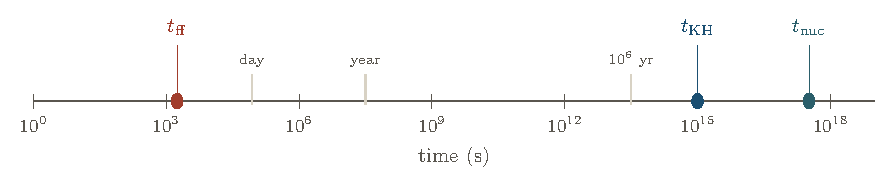
\includegraphics{fig_ch10_clocks.pdf}
	\caption{The free-fall, Kelvin–Helmholtz and nuclear times of the Sun on a logarithmic axis, with a day, a year and a million years for comparison.}
	\label{sg:fig:clocks}
\end{figure}

This ordering is a P6 statement, and it is why a star can be described as a sequence of hydrostatic models. A star restores its balance within an hour, while its heat content changes over tens of millions of years and its composition over billions. At every moment it is in hydrostatic equilibrium, to great accuracy, and it moves slowly from one equilibrium to the next as it loses energy or burns fuel. A collapsing cloud is different. During free fall, $t_{\rm ff}$ is the only clock, the gas is not in balance at any moment, and no equilibrium description holds.

% ==============================================================================
\section{Rotation and the End of Collapse}
\label{sg:sec:rotation}

Free fall assumed a cloud with no pressure, no rotation, and gas that radiates away every bit of heat.

None of these lasts. Real clouds turn a little, and as they become denser they become opaque to their own cooling radiation.

Think of a figure skater spinning with arms held out. When the skater pulls the arms in, the spin becomes much faster. Nothing pushed the skater. The angular momentum stayed the same while the size shrank.

A collapsing cloud does the same (P1 for angular momentum, Section~\ref{pr:sec:p1}). Its spin grows as it shrinks, and the outward pull of rotation grows faster than gravity. Along the axis of rotation nothing resists, so the cloud keeps falling there. Across the axis the spin stops it. The cloud flattens into a disk.

In numbers, the ratio of the rotational pull to gravity grows as $1/R$ (below). A core that shrinks from $0.1\,\mathrm{pc}$ to the size of the Sun raises that ratio by $4\times10^6$. A rotation far too slow to notice at the start becomes the main obstacle at the end.

The picture is a sphere that flattens into a spinning disk with a dense centre.

The same spin-up gives the disks in which planets form, the accretion disks around black holes, the disks of spiral galaxies and the fast spin of young neutron stars. It gives the rotation ratio, the end of the collapse, and the three meanings of equilibrium.

\paragraph{The rotation ratio.} Let a parcel at radius $R$ circle the axis with speed $v_{\rm rot}$, so its angular momentum per unit mass is $Rv_{\rm rot}$, which is conserved. The ratio of the rotational pull to gravity is
\begin{align}
	\frac{v_{\rm rot}^2/R}{GM/R^2}
	&\eqby{1} \frac{v_{\rm rot}^2R}{GM} \nonumber\\
	&\eqby{2} \frac{(Rv_{\rm rot})^2}{GM}\,\frac1R .
\end{align}
\begin{explain}
	\item Rotational acceleration $v_{\rm rot}^2/R$ divided by the gravity of the mass $M$ inside.
	\item Group the conserved angular momentum per unit mass.
\end{explain}
With $Rv_{\rm rot}$ and $M$ fixed, the ratio grows as $1/R$. Shrinking $R$ by some factor raises the ratio by the same factor.

\paragraph{The end of the isothermal collapse.} While the gas can radiate away the heat of compression, its temperature stays nearly constant and the collapse goes on. Once the centre becomes dense enough to be opaque to its own cooling radiation, the heat stays in. The pressure now rises faster than the density, close to an adiabat with $\gamma=\tfrac75$ for molecular hydrogen, above $\tfrac43$. By Eq.~\eqref{sg:eq:E_gamma} a static balance is again possible. The centre stops falling and forms the \textbf{first hydrostatic core}, a few hundredths of a solar mass, which grows by catching the gas still falling in.

The core heats as it grows. Near $2000\,\mathrm K$ the hydrogen molecules start to break apart. Breaking them takes energy that would otherwise raise the pressure, so during this phase the gas behaves as if $\gamma<\tfrac43$. By Eq.~\eqref{sg:eq:E_gamma} no static balance exists, and the core collapses a second time, until the molecules are gone and the gas, now atomic and soon ionised, can stop it again. That second core is the protostar.

\paragraph{Three kinds of equilibrium.} The word equilibrium has been used in three senses, and they differ.
\begin{itemize}
	\item \textbf{Hydrostatic equilibrium} is mechanical. The forces on each parcel balance, Eq.~\eqref{sg:eq:hse}. A star is in it to great accuracy.
	\item \textbf{Global thermodynamic equilibrium} means no net flow of heat anywhere, and in Newtonian physics a single temperature throughout. A star is never in it. Its temperature falls from the centre outward, and that is why energy flows out. (In general relativity the condition is a little different, Section~\ref{cs:sec:relativistic}.)
	\item \textbf{Local thermodynamic equilibrium} means that each small parcel is close to equilibrium inside itself, with one temperature for its gas and its light, even though the temperature changes from parcel to parcel. This holds deep inside stars, and it is what lets the gas pressure and the light of a parcel be written with the formulas of P3. Chapters~\ref{ch:radiation} and~\ref{ch:structure} rely on it.
\end{itemize}
A star can be in excellent hydrostatic equilibrium while far from global thermodynamic equilibrium, and for most of its interior local thermodynamic equilibrium sits between the two.

% ==============================================================================
\section{Problem Set: Self-Gravitating Gas}

\subsection{Problem 1: Scale Heights of Planetary Atmospheres}
\label{sg:prob:scale}

\textbf{Problem Statement}: Find the scale height of (a) the Earth's atmosphere ($T=288\,\mathrm K$, mean molecular mass $28.97\,\mathrm u$, $g=9.81\,\mathrm{m\,s^{-2}}$) and (b) the atmosphere of Mars ($T=210\,\mathrm K$, mostly $\mathrm{CO_2}$ with mean molecular mass $43.3\,\mathrm u$, $g=3.71\,\mathrm{m\,s^{-2}}$). (c) Why is the scale height of Mars larger, although its air is heavier and colder?

\textbf{Essential Ideas}:
\begin{itemize}
	\item Hydrostatic equilibrium with an ideal gas at one temperature gives $H=k_BT/(\mu m_{\rm H}g)$, Eq.~\eqref{sg:eq:scale_height}.
\end{itemize}

\textbf{Detailed Solutions}:
\begin{enumerate}[label=(\alph*)]
	\item \textbf{Earth}. $H=(1.381\times10^{-23}\times288)/(28.97\times1.661\times10^{-27}\times9.81)\,\mathrm m$.
	\[
	\boxed{H_\oplus\simeq8.4\,\mathrm{km}.}
	\]
	\item \textbf{Mars}.
	\[
	\boxed{H_{\rm Mars}\simeq10.9\,\mathrm{km}.}
	\]
	\item \textbf{Comparison}. $H\propto T/(\mu g)$. The heavier, colder air of Mars lowers $H$ by a factor $(210/288)(28.97/43.3)=0.49$, but its weaker gravity raises it by $9.81/3.71=2.6$, which wins.
\end{enumerate}

\subsection{Problem 2: The Temperature of a Galaxy Cluster}
\label{sg:prob:cluster}

\textbf{Problem Statement}: The galaxies of a rich cluster move with a line-of-sight velocity dispersion $\sigma=1000\,\mathrm{km\,s^{-1}}$. The cluster also holds hot ionised gas ($\mu=0.6$) in hydrostatic equilibrium in the same gravitational well. Estimate the temperature of that gas. In which band of light does it shine?

\textbf{Essential Ideas}:
\begin{itemize}
	\item The galaxies and the gas feel the same well, so by the virial theorem their particles have the same kinetic energy per unit mass on average.
	\item For galaxies, the kinetic energy per unit mass is $\tfrac32\sigma^2$ (three directions). For gas, it is $\tfrac32k_BT/(\mu m_{\rm H})$.
\end{itemize}

\textbf{Detailed Solutions}:
Setting the two equal, $k_BT=\mu m_{\rm H}\sigma^2$, so
\[
\boxed{T=\frac{0.6\times1.673\times10^{-27}\times(10^6)^2}{1.381\times10^{-23}}\,\mathrm K\simeq7\times10^7\,\mathrm K.}
\]
Gas at this temperature has $k_BT\approx6\,\mathrm{keV}$ and shines in X-rays, as clusters are observed to. Measuring this temperature and the density profile of the gas, and using Eq.~\eqref{sg:eq:hse}, gives the mass of the cluster, which comes out far larger than the mass in stars and gas. This is the X-ray version of Zwicky's argument for dark matter.

\subsection{Problem 3: Jeans Mass of a Dense Core}
\label{sg:prob:jeans}

\textbf{Problem Statement}: For a molecular core with $\mu=2.33$, find the Jeans mass (a) at $10\,\mathrm K$ and $n=10^{10}\,\mathrm{m^{-3}}$, (b) at $20\,\mathrm K$ and the same density, and (c) at $10\,\mathrm K$ and $n=10^{12}\,\mathrm{m^{-3}}$. What does (c) say about a core that collapses while staying at $10\,\mathrm K$?

\textbf{Essential Ideas}:
\begin{itemize}
	\item Eq.~\eqref{sg:eq:jeans_mass}, with $M_J\propto T^{3/2}\rho^{-1/2}$.
\end{itemize}

\textbf{Detailed Solutions}:
\begin{enumerate}[label=(\alph*)]
	\item \textbf{Reference core}. $\rho=n\mu m_{\rm H}=3.9\times10^{-17}\,\mathrm{kg\,m^{-3}}$ in Eq.~\eqref{sg:eq:jeans_mass}.
	\[
	\boxed{M_J\simeq5.4\,M_\odot.}
	\]
	\item \textbf{Twice as warm}. $M_J$ grows by $2^{3/2}=2.8$.
	\[
	\boxed{M_J\simeq15\,M_\odot.}
	\]
	\item \textbf{A hundred times denser}. $M_J$ falls by $\sqrt{100}=10$.
	\[
	\boxed{M_J\simeq0.54\,M_\odot.}
	\]
	A core that collapses while staying cold has a Jeans mass that keeps falling, so its parts become unstable on their own and it fragments.
\end{enumerate}

\subsection{Problem 4: The Age of the Sun Before Fusion Was Known}
\label{sg:prob:kh}

\textbf{Problem Statement}: In the nineteenth century, Kelvin and Helmholtz assumed the Sun shines by slowly contracting. Estimate how long it could have shone at its present luminosity $L_\odot=3.83\times10^{26}\,\mathrm W$. Compare with the age of the Earth from geology and radioactivity, about $4.5\times10^9$ years.

\textbf{Essential Ideas}:
\begin{itemize}
	\item $t_{\rm KH}=|U|/L$ with $|U|\sim GM^2/R$.
	\item By the virial theorem only half of the released energy is radiated, which changes only the factor in front.
\end{itemize}

\textbf{Detailed Solutions}:
\[
\boxed{t_{\rm KH}\sim\frac{GM_\odot^2}{R_\odot L_\odot}=\frac{6.674\times10^{-11}\times(1.989\times10^{30})^2}{6.957\times10^8\times3.83\times10^{26}}\,\mathrm s\simeq3\times10^7\ \text{years}.}
\]
This is about a hundred times shorter than the age of the Earth. Gravity alone cannot have powered the Sun for that long, which pointed to a much larger store of energy, later found in the nucleus.

\subsection{Problem 5: A Star That Heats as It Cools}
\label{sg:prob:negheat}

\textbf{Problem Statement}: A young star of one solar mass, made of ionised gas with $\mu=0.6$, contracts toward the main sequence. It shines with $L=L_\odot$ for $10^6$ years without any fusion. By how much does its mean temperature change? Does it rise or fall?

\textbf{Essential Ideas}:
\begin{itemize}
	\item The heat capacity of a star in virial balance is $C=-\tfrac32Nk_B$, Eq.~\eqref{sg:eq:negative_C}.
	\item The energy lost is $L\times$ time.
\end{itemize}

\textbf{Detailed Solutions}:
$N=M/(\mu m_{\rm H})=2.0\times10^{57}$, so $C=-4.1\times10^{34}\,\mathrm{J\,K^{-1}}$. The energy lost is $\Delta E=-3.83\times10^{26}\times3.16\times10^{13}\,\mathrm J=-1.2\times10^{40}\,\mathrm J$.
\[
\boxed{\Delta\bar T=\frac{\Delta E}{C}\simeq+3\times10^5\,\mathrm K.}
\]
The temperature rises. The star loses energy and gets hotter, and it keeps contracting and heating until its centre is hot enough for hydrogen to fuse.
